\section{Оптимизация приложений \LB}
\label{sec:optimization}

Коротко остановимся на обзоре тех параметров, которые включает в себя разработка приложений для больших объемов данных, поскольку для этого необходим ряд сложный инженерских решений.

Во-первых, в сложившейся ситуации нет «серебряной пули», то есть невозможно найти единственное универсальное решение, которое идеально ложится и решает все существующие проблемы. Во всяком случае, на данном этапе такого еще не достигли. Можно разбивать на более мелкие детали и пытаться оптимизировать их, но единого подхода и метода сразу для всей системы все же нет. Во-вторых, нет простых решений даже для более мелких компонентов, которые в абсолютном большинстве случаев верны. То есть всякое решение ситуативно – оно имеет свои необходимые условия выполнения. В-третьих, постоянно возникает своеобразное противостояние в выборе между запросами на получение данных и обновление, на real-time выполнение и использование пакетных обработок. Поэтому оптимизация включает в себя выбор таких уступок между потенциальными вариантами решения, что должно, несомненно, учитывать знания того, как \logiql большие структуры данных в выполнение операций.

Как и любая другая отладка, оптимизация представляет собой процесс выявления и устранения неполадок в системе. Это особенный навык, который может быть развит разбором подходящих примеров, следованию дельным советам, изучением нужного материала. Для новичков очень важным методом развития такого навыка является не прямое выявление глубоких (или коренных) причин проблемы, а постепенный систематический сбор информации, проверка локальных гипотез и реакция на их результаты. Вообще говоря, это очень хорошее качество в выявлении проблем экспертов, которые применяют так называемый \emph{breadth-first problem solving}. Такой метод как раз подразумевает детальное рассмотрение множества причин и преднамеренное инвестирование интеллектуальных ресурсов в исследование гипотез с целью избежать перехода к финальным заключениям.

Кроме того, очень важно иметь хорошее понимание доменной области. В противном случае попытки оптимизировать программу могу привести к полному непониманию разработчиков, которые будут иметь дело с измененной реализацией. То есть, оптимизация не должна изменять \emph{логичность} выполнения действий и вычислений.

\subsection{Представление данных на диске}
\label{sec:optimization:data_repr}

Для наглядности и простоты в данном примере используем простую схему и ограничимся тем, что \lstinline{sku}, \lstinline{store}, \lstinline{week} имеют каждый ровно 9
записей:

\begin{lstlisting}[language=Prolog]
sku(s), sku_id(s:id) -> string(id).
loc(l), loc_id(l:id) -> string(id).
week(w), week_id(w:id) -> string(id).
sales[s, l, w]=f -> sku(s), loc(l), week(w), decimal(f).
\end{lstlisting}

Исходя из наших ограничений ключами в sales являются трехразрядные числа: 121, 152. Теперь расссмотрим на рисунке \ref{fig:optimization:data_repr:pages_in_memory}, как записи каждого предиката хранятся с помощью страниц.

\begin{figure}
	\centering
	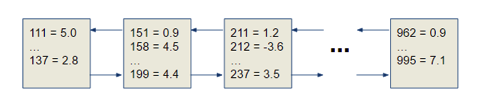
\includegraphics[scale=1.8]{pages_in_memory.png}
	\caption{Пример представления страниц в памяти}
	\label{fig:optimization:data_repr:pages_in_memory}
\end{figure}

Каждая страница хранит упорядоченную последовательность пар ключ/значение. Кроме того, в ней содержатся указатели на следующую и предыдущую страницы для упрощения сканирования страниц. При этом для них необязательно (и в общем случае такое не выполняется) находиться в последовательных блоках памяти и заполненными максимальным количеством пар. Как видно из рисунка, каждая страница в нашем примере содержит лишь значения для одного \lstinline{sku}, поскольку начинаются элементы лишь с определенной цифры, которая по своему месту соответствует как раз параметру \lstinline{sku}.

Эффективной структурой поиска по узлам с помощью таких ключей и указателей является не что иное, как \emph{B+ дерево}, в котором листьями являются страницы с парами ключ/значение. Для краткости и простоты понимания показан лишь один не листовой узел, но в реальности это тоже отдельная страница на диске (на рисунке \ref{fig:optimization:data_repr:page_pointers} горизонтально показана для простоты чтения).

\begin{figure}
	\centering
	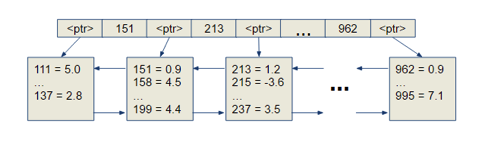
\includegraphics[scale=1.8]{page_pointers.png}
	\caption{Пример использования страницы с указателями}
	\label{fig:optimization:data_repr:page_pointers}
\end{figure}

Теперь посмотрим на запрос:

\begin{lstlisting}[language=Prolog]
_[]=m <-
  agg <<m=max(v) >>
    sku_id(s:"Sprite"),
    loc_id(l:"Belarus")
    sales[s, l, _]=v.
\end{lstlisting}

\lstinline{sku_id}: 1 = \lstinline{Sprite}, ... 9 = \lstinline{Chupa Chups}

\lstinline{store_id}: 1 = \lstinline{USA}, ... 5 = \lstinline{Belarus}, ... 9 = \lstinline{Russia}

Если рассматривать выполнения поиска по шагам:

\begin{enumerate}
  \item инициализируем \lstinline{sku_id} итератор;
  \item двигаем итератор \lstinline{sales} для выравнивания с итератором \lstinline{sku_id};
  \item инициализируем итератор \lstinline{loc_id};
  \item двигаем итератор \lstinline{sales} для выравнивания с итератором \lstinline{loc_id};
  \item считаем агрегированное значение из запроса.
\end{enumerate}


\subsection{Проблемы производительности при операциях случайного добавления}
\label{sec:optimization:random_updates}

Операции случайного добавления (\emph{random insertion updates}) – такие операции обновления предиката с помощью дельта-предиката, которые исходя из упорядоченных ключей в структуре представления на диске затрагивают изменения в слишком большом количестве страниц.

Например, у нас после выполнения недельного скрипта сохранилась информация о продажах за некоторую неделю. Дельты для них:

\begin{lstlisting}[language=Prolog]
^sales["Sprite", "Belarus", "20160917"]=9.6
^sales["Sprite", "Russia", "20160917"]=2.0
^sales["Maple syrup", "Belarus", "20160917"]=4.0
\end{lstlisting}

Посмотрим, что происходит при обновлении предиката \lstinline{^sales}:

\begin{enumerate}
  \item инициализация итераторов (рисунок \ref{fig:optimization:random_updates:iter_init});
  \item выравнивание итераторов – установка на первую страницу (рисунок \ref{fig:optimization:random_updates:iter_align_first});
  \item обновление записи (рисунок \ref{fig:optimization:random_updates:iter_update_fact});
  \item перемещение итераторов далее (рисунок \ref{fig:optimization:random_updates:iter_advance});
  \item обновление следующих записей и т.д.
\end{enumerate}

\begin{figure}
	\centering
	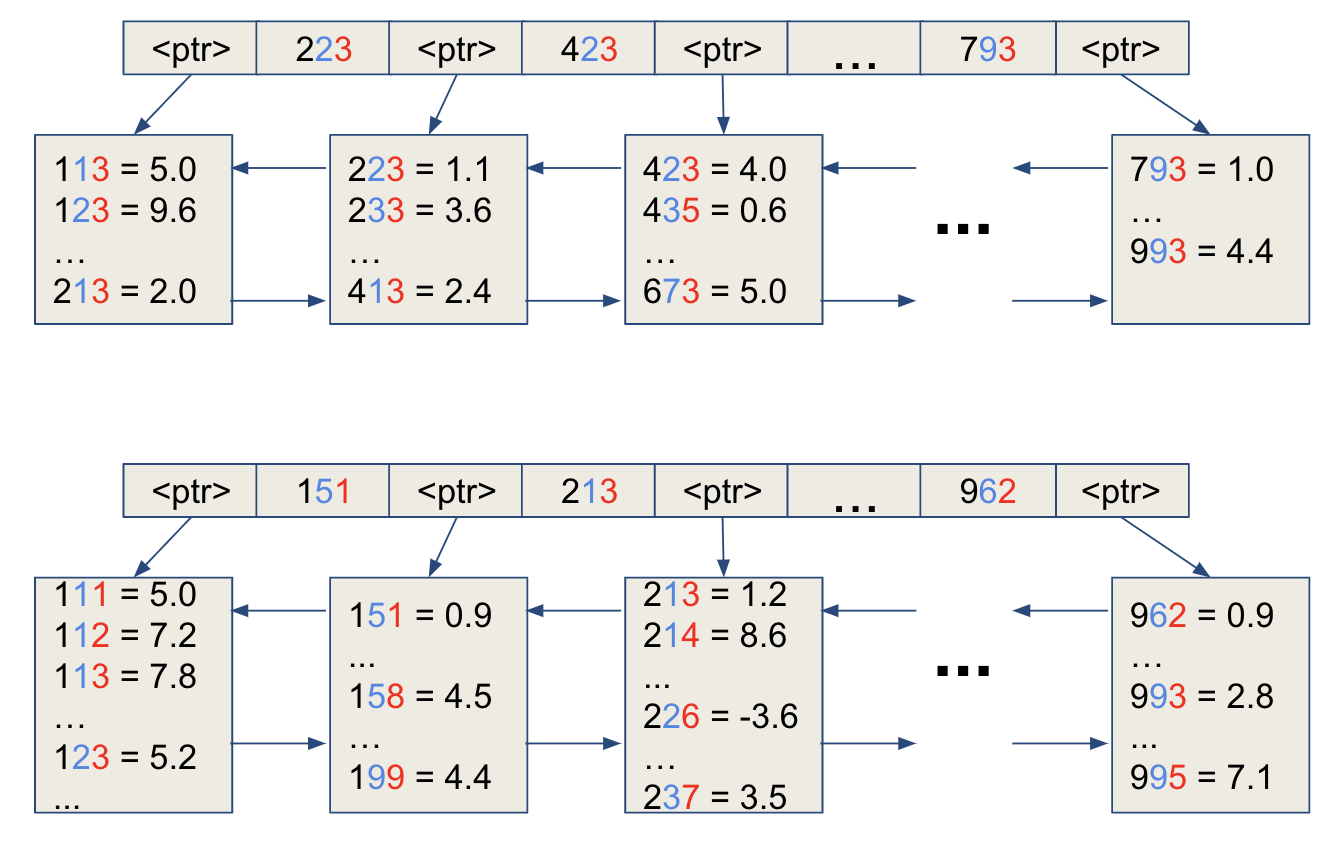
\includegraphics[scale=0.3]{update_0.png}
	\caption{Начальные значения в предикатах \lstinline{^sales} и \lstinline{sales}}
	\label{fig:optimization:random_updates:iter_init}
\end{figure}
\begin{figure}
	\centering
	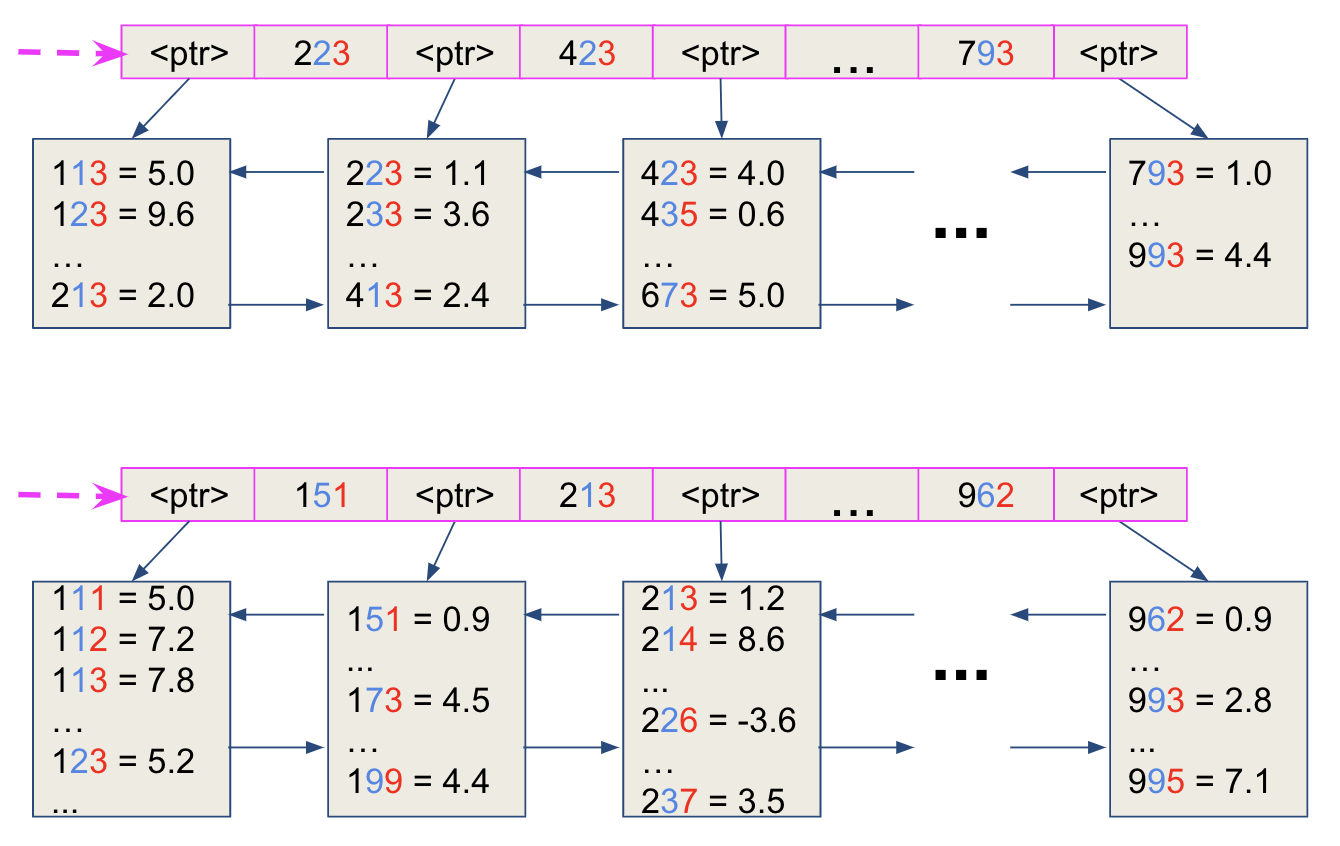
\includegraphics[scale=0.3]{update_1.png}
	\caption{Выравнивание итераторов по первым страницам}
	\label{fig:optimization:random_updates:iter_align_first}
\end{figure}
\begin{figure}
	\centering
	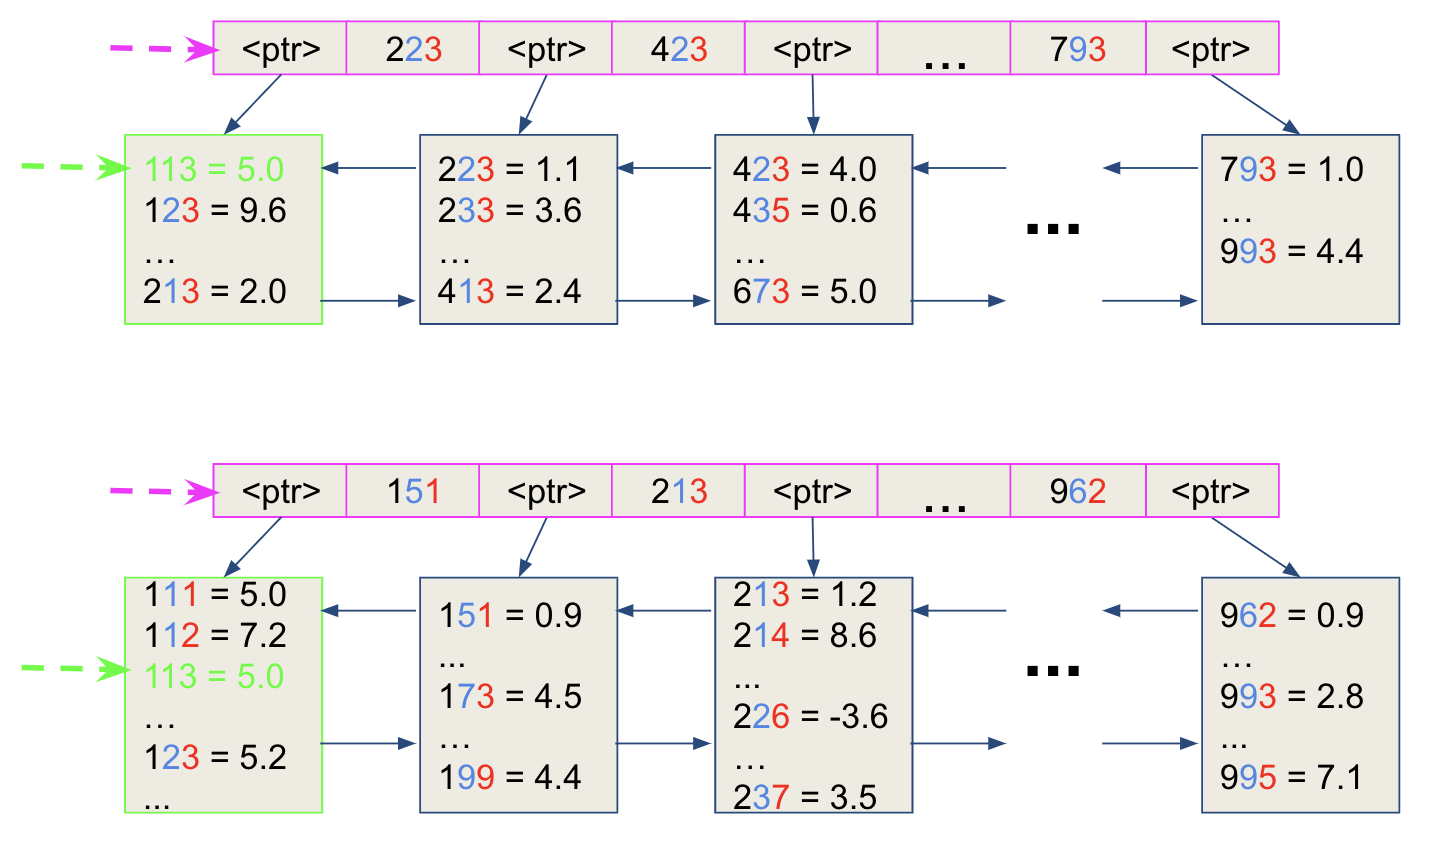
\includegraphics[scale=0.3]{update_2.png}
	\caption{Нахождение нужной записи и ее обновление}
	\label{fig:optimization:random_updates:iter_update_fact}
\end{figure}
\begin{figure}
	\centering
	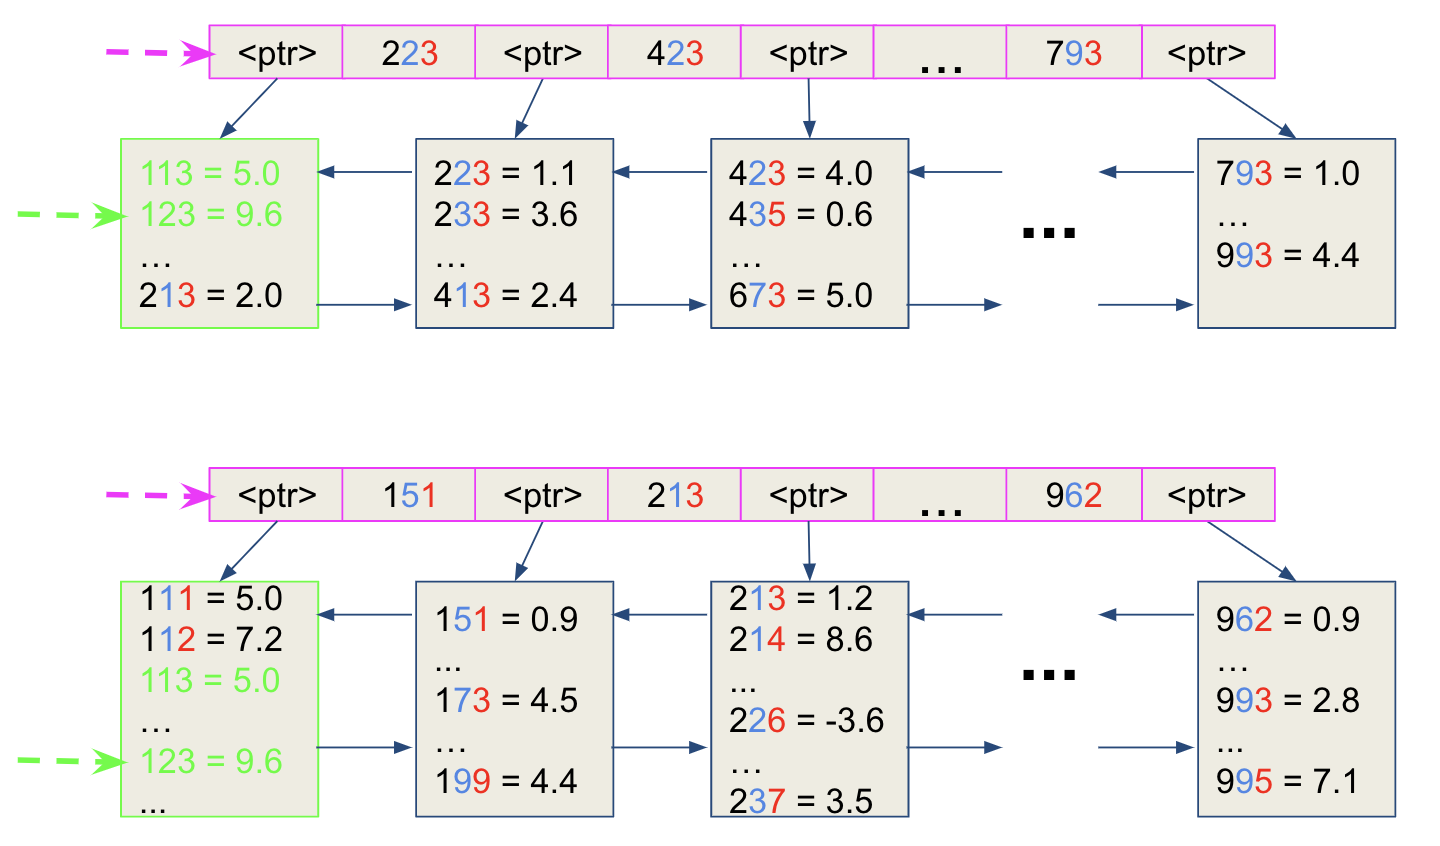
\includegraphics[scale=0.3]{update_3.png}
	\caption{Перемещение итераторов далее для обновления следующих записей}
	\label{fig:optimization:random_updates:iter_advance}
\end{figure}

Из приведенного алгоритма можно увидеть, что при обновлении пришлось пройтись \emph{по всем} страницам. Это может стать проблемой при очень больших предикатах (например, исторические данные о продажах). В таких случаях среда выполнения пытается использовать несколько итераторов, выполняя обновление параллельно (\emph{domain parallelism}). Кроме того, ситуация осложняется при операциях вставки: страницы начинают переполняться, требуя их разбиения и перезаписи. Такое происходит при разовом добавлении большого количества данных.

Разберем на примере описанную ситуацию. Пусть имеется предикат \lstinline{sales[item, location, week] = value}, содержащий историческую информацию о продажах товара в конкретном магазине в каждую неделю. По прошествии очередного интервала времени (недели) в этот предикат необходимо добавить значения о продажах за этот период. Для этого торговая сеть посылает набор файлов (\lstinline{.csv}) с такими значениями, и система начинает вносить их в базу - процесс называется \emph{batch}. В этом случае многие страницы начинают переполняться (потому что пары \lstinline{(item, location)} начинают содержать много данных), что приводит к их перераспределению. В более ранних версиях платформы эту проблему частично решало переупорядочивание ключей в предикате, делая \lstinline{sales[week, location, item] = value}, что не вызывало перезапись существующих страниц, а лишь создание новых (потому что создается новый самый первый ключ). В целом такой подход позволял ускорить время одного "батча" на $40-50\%$.


\subsection{Выполнение операции \join}
\label{sec:technology:join}

Более того, среди возможных проблем производительности – операции \join. Такие операции встречаются довольно часто, в бизнес-\-пра\-ви\-лах их не избежать. Оптимизатор всякий раз выбирает последовательность параметров, по которой ему стоит выполнять \join. Во время операции он использует ключи из тела предиката, эвристически пытаясь отфильтровать данные как можно раньше, чтобы тем самым сократить размер дальнейшей информации для обработки.
Для примера выберем следующий предикат:

\begin{lstlisting}[language=Prolog]
fcst_in_range[sku, store, week] = f <-
  fcst[sku, store, week]=f,
  future_week(week).
\end{lstlisting}

В данном примере возможные (из самых логичных) последовательности объединения – \lstinline{(sku, store, week)}, \lstinline{(week, sku, store)}. Очевидно, что для \lstinline{(sku, store, week)} придется затронуть все страницы для выполнения операции.

Для применения операции из \lstinline{(week, sku, store)} с \lstinline{(sku, store, week)} создается индекс с этой последовательностью ключей. Индексы создаются автоматически, когда это надо.

Наш пример преобразуется в:

\begin{lstlisting}[language=Prolog]
fcst$2_0_1_3[week, sku, store] = f <-
  fcst[sku, store, week] = f.
\end{lstlisting}

После создания индекса, среда выполнит вычисления:

\begin{lstlisting}[language=Prolog]
fcst_in_range[sku, store, week] = f <-
  fcst$2_0_1_3[week, sku, store] = f,
  future_week(week).
\end{lstlisting}

Замечание: приведенные операции выполняются автоматически, то есть все, что может знать разработчик, - можно узнать из логов.

Но с индексами также возможны проблемы:

\begin{enumerate}
  \item При большом количестве операций \join и больших индексах, пользователю приходится ждать завершения материализации индекса.
  \item Индексы все-таки занимают дополнительную память – память увеличивается вдвое, поскольку индекс такой же по размеру, как и предикат, для которого он создается.
  \item Если индекс был создан в \emph{read-only} транзакции, то он не может быть дальше использован после обновления базового для индекса предиката, поскольку данные изменились. В этом случае индекс удаляется при изменении самого предиката. Но, опять же, при постоянных чередующихся запросах на получение результата и изменение предиката, индекс будет создаваться и удаляться каждый раз, что ведет к замедлению работы использования индексов.
\end{enumerate}

С этими проблемами частично справляется пресоздания индексов. Это делается во время дневного скрипта, когда время не играет важную роль. Такие индексы хорошо создавать для тех предикатов, которые не могут быть изменены пользователем, например, предикаты, которые используют прогноз продаж, ведь они используют данные прошлых дней, что является неизменным. Тем самым этот подход стоит лишь дополнительного времени выполнения дневного скрипта и требует больше памяти для хранения, но в целом дает неплохие результаты. Также, абсолютно не рекомендуется создавать такие индексы для больших предикатов, которые обновляется через \ui.


\subsection{Принужденное изменение порядка ключей}
\label{sec:optimization:key_ordering}

Для понимания текущей проблемы стоит рассмотреть пример:

\begin{lstlisting}[language=Prolog]
fcst_in_range[sku, store, week] = f <-
  fcst[sku, store, week]=f,
  future_week(week).
\end{lstlisting}

Поскольку одной из идей платформы является выполнение операции \join сразу по всем ключам, то оптимизатор запроса должен выбрать необходимый порядок ключей, чтобы выполнить фильтрацию, в случаях выполнения или поддержания правила. В качестве ключей выступают все переменные в выражениях в теле правила. Алгоритм является эвристическим и направлен на то, чтобы как можно раньше отфильтровать объекты. Этот подход легко объясняется - чем раньше происходит фильтрация, тем меньше данных нужно будет обработать для выполнения \join. Возможные следующие варианты порядка ключей:

\begin{itemize}
  \item \lstinline{[sku, store, week]};
  \item \lstinline{[week, sku, store]};
  \item могут быть другие варианты, но они, очевидно, хуже.
\end{itemize}

На рисунке \ref{fig:optimization:key_ordering:key_ordering_choice} представлен пример размещения страниц с данными для предиката \lstinline{fcst_in_range}. Далее, на рисунке \ref{fig:optimization:key_ordering:key_ordering_choice_join}, уже показана попытка сделать \join для ключа \lstinline{week}. Как видно, чтобы это осуществить, необходимо проитерироваться \emph{по всем} страницам предиката, поскольку ключ \lstinline{week} идет в нем последним. Поэтому выбор порядка ключей \lstinline{[week, sku, store]} неудачен и оптимизатор сделает предпочтение \lstinline{[sku, store, week]}.

\begin{figure}
	\centering
	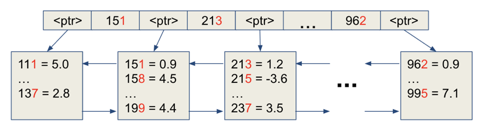
\includegraphics[scale=0.9]{key_ordering_choice.png}
	\caption{Пример представления страниц в памяти для предиката \lstinline{fcst_in_range}}
	\label{fig:optimization:key_ordering:key_ordering_choice}
\end{figure}

\begin{figure}
	\centering
	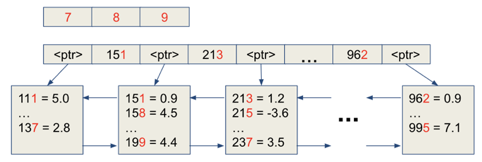
\includegraphics[scale=0.9]{key_ordering_choice_join.png}
	\caption{Выполнения операции \join по ключу \lstinline{week}}
	\label{fig:optimization:key_ordering:key_ordering_choice_join}
\end{figure}

Рассмотрим следующую проблему. Пусть в некотором предикате (в силу решения проблемы случайных вставок) порядок ключей определен как \lstinline{[week, sku, store]}, а в другом - \lstinline{[sku, store, week]}, и их необходимо слить. Для этого необходимо воспользоваться индексом. В данном случае понадобится инвертированный индекс \cite{inverted_index}, который позволит одному из предикатов перейти к другому порядку ключей. Такой индекс создается \emph{автоматически} исполняющей средой, если на то есть необходимость. Из плюсов:

\begin{itemize}
  \item помогает быстро отвечать на запросы разного порядка ключей.
\end{itemize}

Минусы:

\begin{itemize}
  \item его необходимо поддерживать (дублировать data modification операции с исходного предиката);
  \item он занимает столько же памяти, сколько и исходный предикат.
\end{itemize}

Рассмотрим пример. При выполнении кода выше среда может добавить инвертированный индекс, и правило перезапишется следующим образом:

\begin{lstlisting}[language=Prolog]
fcst_in_range[sku, store, week] = f <-
   fcst$2_0_1_3[week, sku, store] = f,
   future_week(week).
\end{lstlisting}

Здесь инвертированный индекс \lstinline{fcst$2_0_1_3} (такие индексы всегда имеют такие названия с порядком ключей, чтобы давать информацию о себе, встречая его впервые и не лезя в детали) выглядит так:

\begin{lstlisting}[language=Prolog]
fcst$2_0_1_3[week, sku, store] = f <-
  fcst[sku, store, week] = f.
\end{lstlisting}

Создание и использование индексов скрыто от разработчика - это все решает среда выполнения. Чтобы отыскать детали использования индексов, стоит смотреть в специальные логи.

Как и в других ситуациях, решение с индексами не дает исключительных выгод. Есть и серьезные недостатки:

\begin{enumerate}
  \item Поскольку они создаются автоматически (разработчик не может это контролировать), при некоторых долгих запросах пользователь может ждать дольше, чем обычно, из-за создания индекса.
  \item Как упоминалось, индексы занимают примерно столько же памяти, сколько и исходные предикаты.
  \item В некоторых случаях, когда индекс создается в readonly транзакциях, он не будет поддерживаться в дальнейшем при изменениях исходного предиката. В таких ситуациях индекс удаляется при следующей операции изменения, что занимает временные ресурсы. Поэтому если изменять большой по размеру предикат, а затем делать на нем запросы, требующие индекса, такой индекс будет создаваться и удаляться каждый раз.
\end{enumerate}

Управление индексами в процессе выполнения скрыто для разработчика. Единственное, что можно сделать, это создание индексов заранее. Такое решение оправдано, когда заранее можно быть увереным, что среда будет часто пересоздавать индекс, либо просто выгодно создать его именно во время разворачивания всей системы, а не в процессе выполнения. Для этого индексы описываются в специальном файле \lstinline{scripts/indexes.txt}. Среди проблем такого подхода:

\begin{itemize}
  \item использование индекса замедляет обновления;
  \item скорее всего с ними порядок ключей будет выбран неподходяще.
\end{itemize}

Исходя из таких рассуждений можно вынести следующие рекомендации:

\begin{enumerate}
  \item стоит заранее создавать индексы на предикаты, которые не обновляются с \ui;
  \item индексирование большого предиката, которые обновляется с \ui - очень плохая идея;
  \item чтобы избавить от необходимости создавать индексы, стоит прибегнуть к переупорядочиванию ключей в теле предиката, но такое решение требует тщательного тестирования.
\end{enumerate}

Чтобы помочь системе правильно использовать индексы, можно подсказывать ей и изменять порядок используемых ключей. Рассмотрим на примере:

\begin{lstlisting}[language=Prolog]
filtered_fcst[sku, store, week]=f <-
  forecast[sku, store, week]=f,
  filter(sku, store),
  fcst_horizon(week).
\end{lstlisting}

И наложим ограничения (для примера):

\begin{itemize}
  \item \lstinline{fcst_horizon} содержит 52 записи (текущая неделя и на год вперед);
  \item \lstinline{filter} содержит 100.000 записей, но довольно разрежен по параметру \lstinline{sku};
  \item оптимизатор выберет порядок ключей как \lstinline{(week, sku, store)}. Заранее скажем, что это плохой выбор порядка ключей, так как кроме построения индекса, \lstinline{filter} по факту не сделает большой работы по самой фильтрации.
\end{itemize}

Итак, исходя из некоторых соображений (возможно, мы знаем, как предикаты могут фильтровать друг друга, или мы хотим не давать системе создавать большой индекс), мы создаем прагму:

\begin{lstlisting}[language=Prolog]
pragma_force_key_ordering(sk, st, wk) ->
  sku(sk), loc(st), week(wk).
\end{lstlisting}

Прагма явно задает порядок ключей, который оптимизатор должен выбрать. Теперь мы можем использовать данную прагму в нашем правиле:

\begin{lstlisting}[language=Prolog]
fcst_in_range[sku, store, week] = f <-
  pragma_force_key_ordering(sku, store, week),
  fcst[sku, store, week]=f,
  filter(sku, store),
  future_week(week).
\end{lstlisting}

В этом случае, оптимизатор однозначно определит порядок ключей как \lstinline{[sku, store, week]}. Более того, как описывалось в главе \ref{sec:technology:web_services:tdx}, в \tdx сервисе платформа сама неявно создает дополнительные правила и предикаты. В этом случае, порядок ключей также может быть выбран неправильным, если идет большой \join по многим ключам. Это отлавливается на очень долгих выполнениях импорта/экспорта данных. В таких ситуациях применяется следующий хак: в конфигурацию \tdx сервиса в качестве одного из предикатов для фильтрации (\join) добавляется необходимая прагма. Тогда в созданное платформой правило она подставится автоматически, а дальше оптимизатор подхватит ее и выберет указанный порядок ключей. Например в секции \emph{File binding} можно указать следующую конструкцию:

\begin{lstlisting}[language=Prolog]
binds_pred["pragma_force_key_ordering"]="SKU,STORE,WEEK".
\end{lstlisting}

Теперь оптимизатор выберет порядок ключей \lstinline{(sku, store, week)}. Такой прием особенно полезен при попытках фильтрации с предикатом с меньшим количеством ключей.

Но, как ни странно, широкое использование прагм может привести к ухудшению ситуации:

\begin{itemize}
  \item все-таки это ограничение на оптимизатор, и в большинстве случаев оптимизатор использует более правильный подход;
  \item следует избегать при существовании другого решения;
  \item обычно стоит переформулировать правило и использовать новый материализованный предикат вместо изменения порядка ключей.
\end{itemize}


\subsection{Переформулировка правил для увеличения производительности}
\label{sec:optimization:data_repr:rule_split}

Самый оптимальный способ выполнения правил – это тот, при котором в каждом предикате в теле правила является каким-либо префиксом головы правила.

\begin{lstlisting}[language=Prolog]
filtered_fcst[sku, store, week]=f <-
  fcst[sku, store, week]=f,
  filter(sku, store),
  active(sku).

filtered_fcst[sku, store, week]=f <-
  fcst[sku, store, week]=f,
  filter(sku, store),
  future_week(week).
\end{lstlisting}

Также правильно использовать дельты для того, чтобы сузить количество охватываемой информации во время фильтрации. Если такого свойства нет, то система создает так называемые индексы чувствительности. Они материализуют записи из оригинальной операции объединения, чтобы запомнить регионы в голове предиката, которые можно «запаковать».

Разберемся подробнее. Возьмем пример:

\begin{lstlisting}[language=Prolog]
short_sku_alert(promo, sku) <-
  contains(promo, spot),
  promotes(spot, sku),
  starts_on[promo]=day,
  projected_iventory_of[sku, day] < stock_threshold[].
\end{lstlisting}

Данное правило будет довольно трудоемким в плане выполнения, потому что нет переменной, по которой можно объединить каждый предикат в теле правила. Тогда какой же порядок ключей следует взять?

Попробуем материализовать объединения предикатов, которые скорее всего не будут обрабатываться в качестве ответа на действия пользователя. Такие предикаты могут быть сохранены во время дневного скрипта и только единожды. Более того, если мы таким образом сможем избавиться от переменной, то время обработки запроса увеличится. Теперь нужно ответить на вопрос: какие объединения будут высчитаны один раз во время выполнения скрипта, основываясь на знании информации, которую содержат эти предикаты?

Переформулируем наше правило:

\begin{lstlisting}[language=Prolog]
skus_on_promo(promo, sku) <-
  contains(promo, spot),
  promotes(spot, sku).

short_sku_alert(promo, sku) <-
  skus_on_promo(promo, sku),
  starts_on[promo]=day,
  projected_iventory_of[sku, day] < stock_threshold[].
\end{lstlisting}

\lstinline{skus_on_promo} теперь может быть изменено во время скрипта, при этом этот предикат убирает лишнюю переменную (\lstinline{spot}) из области видимости оптимизатора во время выполнения объединения. Неплохое начало!

Теперь, попробуем увидеть «разреженные фильтры», то есть попробуем вынести в отдельный предикат те данные, фильтрация по которым скорее всего отсечет большое количество записей. Что из этого стоит выбрать?

\begin{lstlisting}[language=Prolog]
shortages(sku, day) <-
  projected_iventory_of[sku, day] < stock_threshold[].

short_sku_alert(promo, sku) <-
  skus_on_promo(promo, sku),
  starts_on[promo]=day,
  shortages(sku, day).
\end{lstlisting}

Данная оптимизация не только отсекает большое количество информации при фильтрации, но и позволяет создать индекс чувствительности по \lstinline{(sku, day)} вместо \lstinline{(promo, sku, day)}.

Но и это еще не все. Попробуем материализовать то объединение, которое применяет разреженный фильтр для удаления переменной из более большого объединения.

\begin{lstlisting}[language=Prolog]
skus_short_at_start(promo, sku) <-
  starts_on[promo]=day,
  shortages(sku, day).

short_sku_alert(promo, sku) <-
  skus_on_promo(promo, sku),
  skus_short_at_start(promo, sku).
\end{lstlisting}

В итоговом варианте в теле правила используется лишь 2 предиката, у которых один и тот же порядок ключей, что дает выигрыш в производительности примерно в 10 раз.


\subsection{Выводы}
\label{sec:optimization:notes}

\begin{itemize}
  \item компилятор переписывает сложные формулы с функциональными предикатами и операторами сравнения в атомарные инструкции;
  \item выбранный порядок ключей при операциях \join часто является причиной длительных запросов (long-running rules). Такие случаи легко выявить при изучении ключей в исходном правиле;
  \item некоторые правила выходят за рамки линейной асимптотики, что плохо сказывается на производительности из-за большого количества исходных данных;
  \item следует избегать правил, которые делают \join по временным объектам, используя неравенства. Вместо этого лучше использовать конструкцию \lstinline{int:range};
  \item стоит хорошо называть промежуточные предикаты, введенные для оптимизации, а также добавлять соответствующие комментарии к ним, чтобы с течением времени эти изменения не были удалены и по-прежнему были понятны;
  \item при использовании \lstinline{force_key_ordering} pragma стоит ставить меньше ключей, чтобы меньше ограничивать оптимизатор;
  \item полезно придерживаться одного шаблона при pragma, например часто используется следующий формат: $"pragma" + $ \lstinline{string} $ +$\linebreak $ "force\_key\_ordering"$;
  \item запись в логах, содержащая \lstinline{long-running "ExUnRule"}, указывает на блок и номер строки с самой long-running rule;
  \item чтобы вывести самые долгие правила, необходимы выполнить \lstinline{grep took lb-server.log |}\lstinline| awk '{print $(NF-1) " " $0;}'|\lstinline{ | sort -r -n|}
  \item настройка окружения \lstinline{LB_SUPPRESS_TASK_PARALLELISM=1} помогает логу быть в едином потоке, в противном случае записи будут находиться в хаотичном порядке;
\end{itemize}

